
% AA vers. 9.0, LaTeX class for Astronomy & Astrophysics
% demonstration file
%                                                       (c) EDP Sciences
%-----------------------------------------------------------------------
\documentclass{aa}
\usepackage{graphicx}
%%%%%%%%%%%%%%%%%%%%%%%%%%%%%%%%%%%%%%%%
\usepackage{txfonts}
\usepackage{subfigure}
%\usepackage{amssymb}
%%%%%%%%%%%%%%%%%%%%%%%%%%%%%%%%%%%%%%%%
%\usepackage[options]{hyperref}
\usepackage{hyperref}
% To add links in your PDF file, use the package "hyperref"
% with options according to your LaTeX or PDFLaTeX drivers.


\begin{document}


   \title{Test of source selection to construct a more stable reference frame}

   \author{N. Liu
          \and
          J.-C. Liu
          \and
          Z. Zhu}

   \institute{School of Astronomy and Space Science \& Key Laboratory of Modern Astronomy and Astrophysics (Ministry of Education), Nanjing University, 210093 Nanjing, China\\
              \email{jcliu@nju.edu.cn}
             }

   \date{Received ; accepted }

  \abstract
  % context heading (optional)
  % {} leave it empty if necessary
   {The International Celestial Reference System (ICRS) is widely used in astronomical research since its adoption by the IAU in 1998. The latest realization of the ICRS in 2010, namely the ICRF2 catalogue, contains 295 well observed radio sources by which the axes of the inertial reference system are defined.}
  % aims heading (mandatory)
   {We aim to evaluate the possibility of improving the ICRS realization starting from the ICRF2 by investigating the time series of radio sources observed by VLBI between 1979 and 2016.}
  % methods heading (mandatory)
   {Sources with long and stable observation are selected as the candidates and least squares fits with special handling of the weights are performed to derive the linear drifts of the coordinates $\alpha\cos\delta$ and $\delta$. Then the sources are ranked based on the normalized linear drift over the whole sky and within four homolographic areas divided by declination. The axial stability of the reference system and sky distribution defined by the selected set of sources are evaluated as the criterion for the final source lists.}
  % results heading (mandatory)
   {As a result, four possible sets of sources are selected to be more suitable for defining a stable celestial reference system compared to the ICRF2, the number of sources being 307, 366, 304 and 324. The global rotation of the axes derived from apparent motion of the sources are about 5 times better than the ICRF2, and the distribution is also more homogeneous.}
  % conclusions heading (optional), leave it empty if necessary
   {}

   \keywords{
                astrometry --
                reference systems --
                Earth
               }

   \maketitle
%-------------------------------------------------------------------
\section{Introduction}
In 1994 the International Astronomical Union (IAU) recommended the adoption of the International Celestial Reference System (ICRS, \cite{Arias1995}), realized by the highly precise coordinates of a specific set of extragalactic radio sources observed at radio wavelength with the Very Long Baseline Interferometry (VLBI), known International Celestial Reference Frame (ICRF). The first version of the ICRF (hereafter referred to as ICRF1) was proposed by \cite{ma1998}, based on 212 defining sources with a positional accuracy batter than 1 milli-arcsecond (mas) in both coordinate. However, as pointed out by the authors, there are some unknown physical characteristics of radio sources, causing a large drift of coordinates. Several subsequent studies on assessing the positional stability for individual sources and the celestial frame axes were carried out \citep[see][]{Feissel2000,AMGontier2001,FV2003,FV2006,gontier2008,Lambert2009}. Some ensembles of sources were proposed, showing a better positional time stability for individual sources and improved overall stability of the reference frame.

In 2009 the updated version of the ICRF (hereafter referred to as ICRF2) was developed, which includes 3414 sources and 295 defining sources therein \citep{2009ITN....35....1M,IERS2}. The ICRF2 improves the stability of axes by a factor about 2 compared to the ICRF1 and with more sources in the southern hemisphere selected, therefore has a more uniform sky distribution. But the time stability estimation of the ICRF2 axes, especially in post-ICRF2 observations, should be continued. In a recent paper, \citep{Lambert2013} shows that there is no significant deformation of the ICRF2 axes by studying the yearly differential reference frames, but the author suggested that such work should be undertaken regularly as the time series updates. After more than 7 years since the publication of the ICRF2, it is necessary possible to investigate if updates of the source selection is necessary, thanks to longer time interval of VLBI observations.

In fact, the selection of sources to construct a reference frame is always complicated and delicate, which is related to the apparent and intrinsic characteristics of the sources in many aspects. Several criteria for choosing sources were adopted in the previous studies. Three aspects of radio sources were mainly investigated in the work for ICRF1 \citep{arias2004,ma1998}: (1) quality of data and observational history, (2) consistency of coordinates derived from subsets of data, and (3) repercussions of source structure. Based on these criteria, sources are categorized into three class: defining, candidate, and other. A method of selecting sources based on the analysis of time series stability of astrometric positions was initially proposed by \cite{FV2003} and the work has been extended in \cite{FV2006}. A similar selection scheme can be found in \cite{gontier2008,Lambert2009}. Several parameters of time series were tested in these works, i.e., standard deviation, slope, Allan standard deviation and goodness of fit, while session time series and regular time series(for example, one-year average) show different statistical characteristics. The selection of the ICRF2 defining sources also partly depend on the time series \citep{2009ITN....35....1M,IERS2} of source coordinates. A stability criterion based on overall positional index and successive structure index were applied according to which the sources were ranked from the most stable to the least. To achieve more uniform sky coverage, loose threshold was set for sources in the southern hemisphere.

In this paper, time series of coordinates are used to select suitable sources. The principle strategy is to obtain new source list by eliminating unstable sources from and adding new stable sources to the current 295 ICRF2 defining sources. The observational history of the sources is considered in Sect.\ref{sect:preselection}, while a detailed description of the selection schemes is given in Sect.\ref{sect:select}. Sect.\ref{sect:conclusion} presents some conclusions.

\begin{figure*}[htb]
   \centering
   \subfigure[]{\includegraphics[width=0.45\hsize]{figures/Observation_span}}
   \subfigure[]{\includegraphics[width=0.45\hsize]{figures/Number_of_session}}
      \caption{Statical histograms of length of the observation span ($left$) and amount of the observational session for a individual source ($right$), displaying the observational histories of the 3826 sources.
              }
         \label{Fig:Observation}
   \end{figure*}

For comparison, several ensembles of sources proposed in the previous studies are used. For clarity, in the following sections, the ICRF1 and ICRF2 defining sources will be referred to as "212ICRF" and "295ICRF" respectively, while the subset of 247 sources provided by \cite{FV2006} will be denoted as "247MFV".
% and the one of 260 sources proposed by \cite{Lambert2009} as "260AMS" (A emsemble of 262 sources was proposed in the paper, but only 260 sources are contained in the available sources list file.).
%--------------------------------------------------------------------
\section{Data and Pre-selection}\label{sect:preselection}
The data used in our study is the VLBI derived coordinate time series for 3826 sources provided by IVS analysis center operated at Paris Observatory\footnote{http://ivsopar.obspm.fr/radiosources/} (\citep[see][Sect.~2 for details]{Lambert2013}).  Figure \ref{Fig:Observation} presents the observational history of the total 3826 sources and the list is labeled as "OPA3826". We note that some non-defining sources have been observed for a longer period and more frequently than some defining ones. This motivates us to check weather more well observed stable sources are qualified for being select as defining sources.

Previous studies \citep[for example]{Lambert2009,AMGontier2001} mentioned that the quality and precision of pre-1990 VLBI data is worse compared to that of the later, therefore the data before 1990.0 should be used with caution. For this reason some of the studies used the coordinate time series only after 1990.0. However, the the ICRF2 working group \citep{IERS2} claimed that the positions and corresponding uncertainties generated from the entire available VLBI observations can represent realistically how confident to use these positions in the future. For this reason, the full available time series from August 1979 up to now will be used in the following.

To exclude sources with a poor observational history or questionable behaviors, a pre-selection algorithm is applied. First, 39 special handling sources with known significant positional instability, 3 known gravitational lenses, and 6 known radio stars\citep[see][Sect.~4]{2009ITN....35....1M} are excluded. Then sources are considered as well observed, only when the interval of observation is longer than 10 years and number of sessions is larger than 20. This threshold is artificial since there is no specific definition of a rich or poor observation history. However taking this kind of filter enables us to keep enough sources for the following studies and at the same time to eliminate very poor observed sources. It should be noted that the time series for a part of ICRF2 defining sources become obviously denser after 2009, most of them being located in the southern hemisphere. These southern sources are kept by our criterion of pre-selection. More strict constrains are tested and most of them will excluded. This is not our wish that more sources in the southern hemisphere should be added to make the reference frame more uniform. Finally, 613 sources including 291 ICRF2 defining sources are retained as candidates for the next step. Four ICRF2 defining sources (1448-648, 1554-643, 1611-710, 1633-810) are ruled out because of too few data points. The source names used here are the IERS source designations. The observational histories of 613 candidate sources are shown in Fig. \ref{Fig:ObsHis}. At low declination zone, several non-defining sources are observed quite frequently, hence are possibly to be selected as defining sources.

\begin{figure}
   \centering
   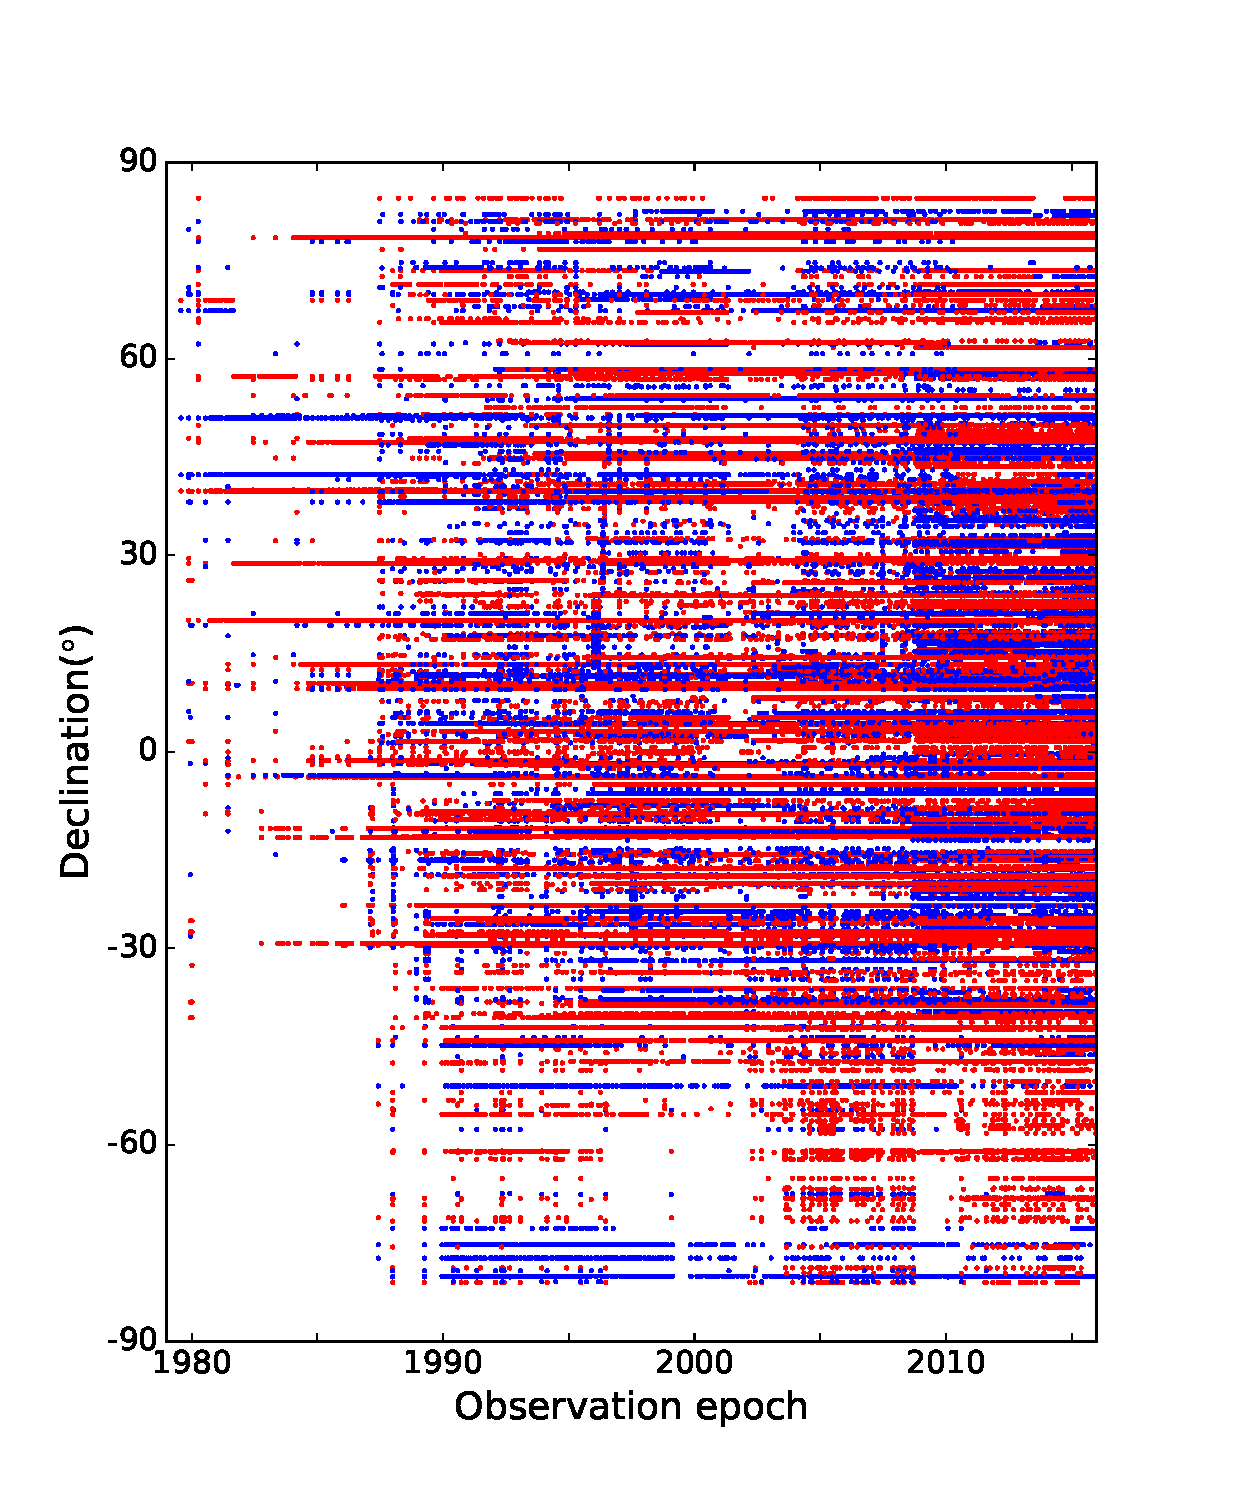
\includegraphics[width=\hsize]{figures/Observation_history.eps}
%	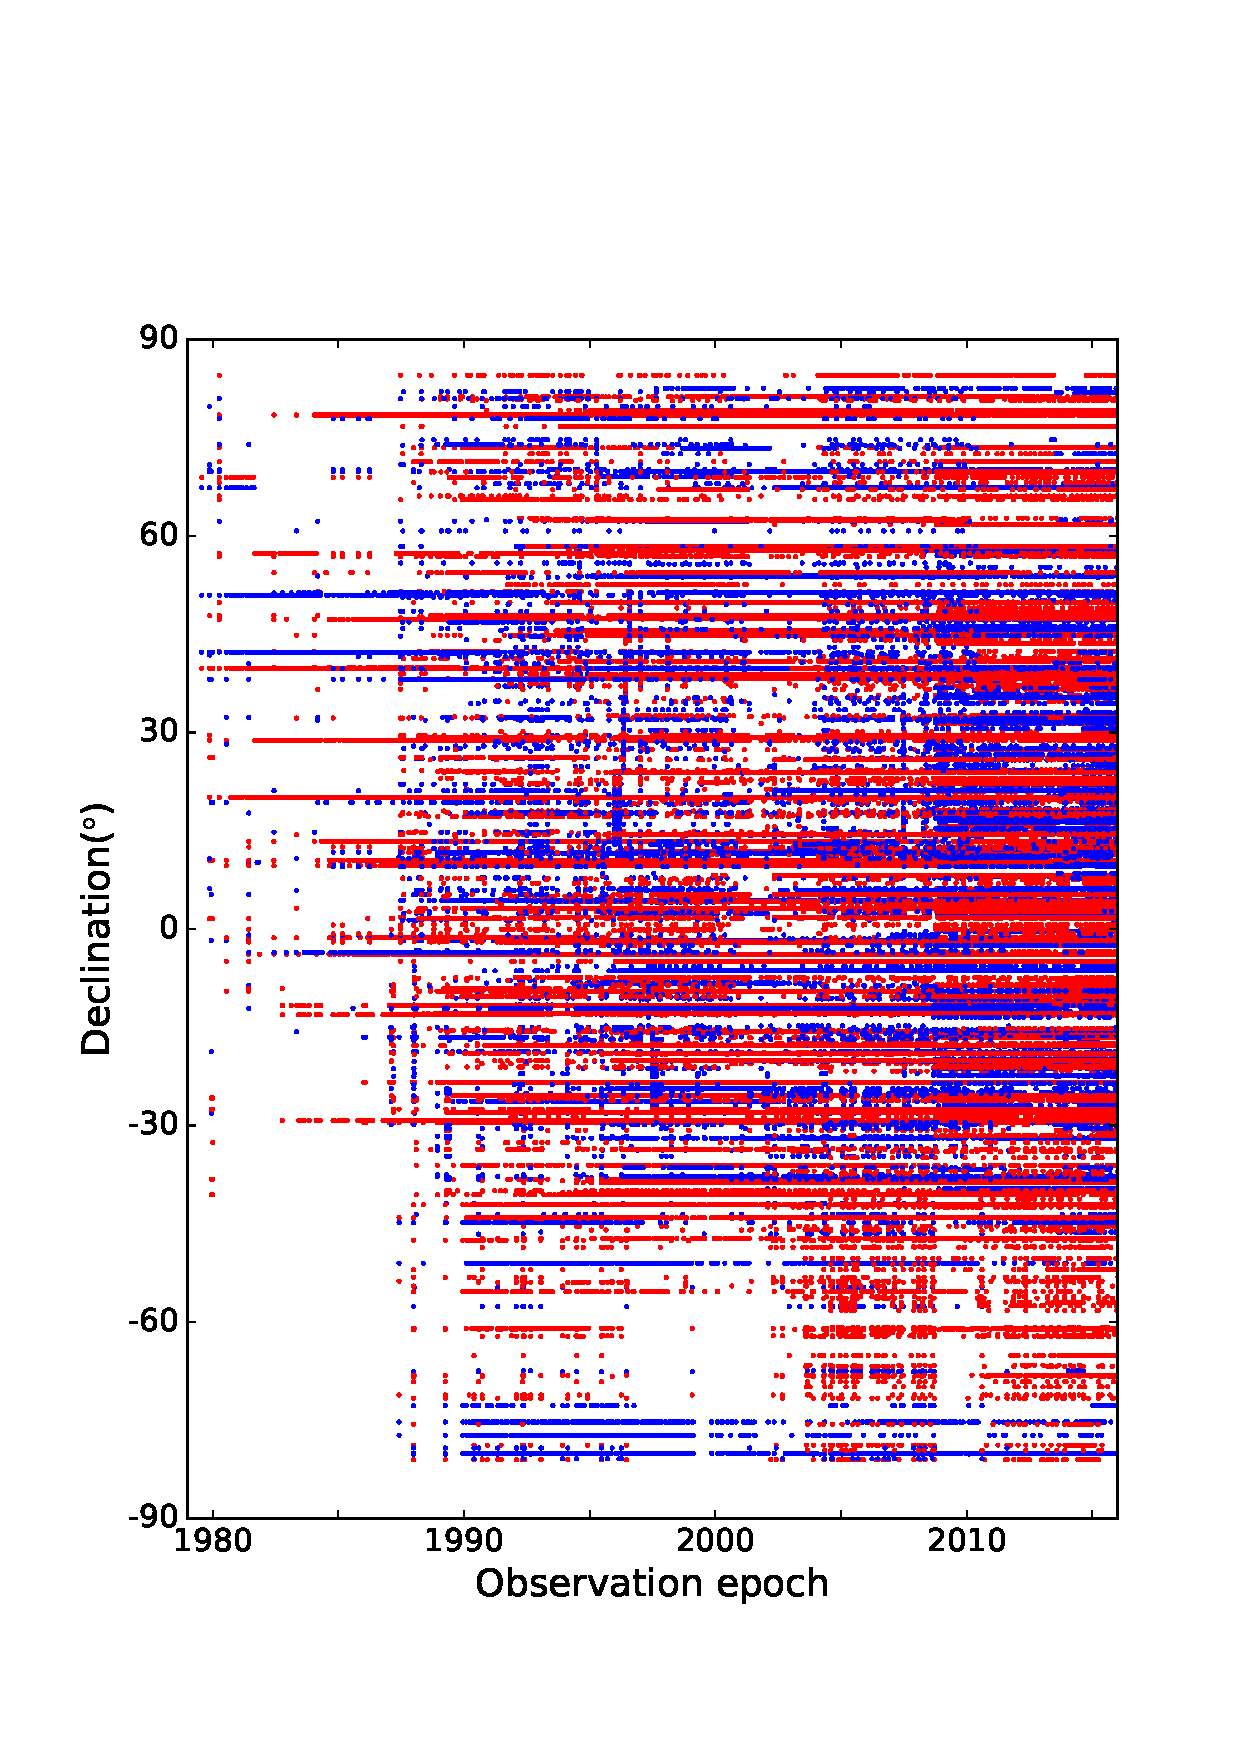
\includegraphics[width=\hsize ,bb=0 0 1440 1080]{figures/Observation_history.PNG} 1
      \caption{
      Observational history of 613 candidates, including 291 ICRF2 defining sources (red points) and 322 non-defining sources (blue points).
              }
         \label{Fig:ObsHis}
\end{figure}

%-----------------------------------------------------------------
\section{Sources Selection}\label{sect:select}
In principle, the extragalactic radio sources are stationary on the celestial sphere without any transversal velocity (proper motions) due to their extremely far distances at the level of Mpc, the time series of coordinates still would show variability owing to, the extend structure, immediate rejection of jet from the central galaxy, and stochastic uncertainties or systematic errors in the observations. All of these physical and observational effects are reflected in the data of source positions, which can be described by certain statistical parameters. That's the reason why we apply the VLBI time series of source coordinates to estimate individual and global behaviors of selected sources, for the purpose of upgrading the ICRF.

In this work, three parameters for the source coordinates $\alpha* = \alpha\cos\delta$ and $\delta$ are used: (i) the weighted standard deviation referred to the mean (weighted root mean square), (ii) the weighted Allan deviation, and (iii) the normalized linear drift (the ratio of linear drift to its uncertainty) from least squares fits. The standard deviation describes the scatters of the coordinates while the Allan deviation shows the stochastic properties of the time series and is sensitive to abrupt changes of source positions. Combination of these two parameters helps us to eliminate sources with significantly noisy time series. With enough data points, the fitted linear drift is considered as the indicator for long-term variation. According \emph{The linear drift estimation is based on an underlying physical assumption, and considered as reliable since time series of these candidates have enough points.}

%In this work, the weighted standard deviation and the weighted Allan deviation are estimated to rule out s while the normalized linear drift  is used as an indicator of positional stability, according to which the sources are ranked from most stable to less in the next procedure.

To derive the Allan deviation of time series, weighted annual average points are calculated contained in an one-year interval over 1980.0-2016.0. \emph{However, few sources have observational histories dense enough for the Allan deviation test.} The method for calculating Allan deviation proposed by \cite{Malkin2008} (labeled as "WADEV" in that paper) is used.

Fig. \ref{Fig:Dev} presents the weighted standard deviation and the weighted Allan deviation of 631 candidate sources. We note that the results are much larger compared to that of \cite{FV2003}. The possible reason is that the entire time series are taken into account while only post-1990.0 time series were used in \citep{FV2003}. Then the sources with the weighted standard deviation or the weighted Allan deviation of both coordinates larger than $10\,\rm{mas}$ are excluded. The number of remaining sources is 499.

The linear drifts $(\mu _{\alpha}\cos\delta\,,\mu_\delta)$ (they have the same unit as proper motion) are obtained using a weighted least squares fit, but with a slightly different way of handling weights. The time series are divided into three observation spans: 1979.0$\sim$1990.0, 1990.0$\sim$2009.0, and 2009.0$\sim$2016.0 on the assumption that each observation span corresponds to discrepant accuracies. The first interval is considered as it contains relative inaccurate source positions, while the last interval is isolated in order to estimate the effect of post-ICRF2 data. The average weight is used as equal weight of session points within the corresponding time span. The normal equations of estimation of $\alpha\cos\delta$ coordinate is given by (\ref{eq:normal}) and the one for $\delta$ coordinate is similar.
\emph{Consider that the formal error contained in time series may include some model error during the data reduction and not represent the real observational error, average weight over a observational span is used.}
\begin{equation}
\label{eq:normal}
\left(
	\begin{array}{c}
	\mu _{\alpha ^{*}} \\
	\alpha ^{*}_0
	\end{array}
\right)
	= \sum _{i=1}^3
\left(
	\begin{array}{cc}
	\sum\limits _j \dfrac{(\Delta t_{ij} )^2}{\sigma ^2_{ij}} & \sum\limits_j \dfrac{(\Delta t_{ij})}{\sigma ^2_{ij}} \\
	\sum\limits_j \dfrac{(\Delta t_{ij})}{\sigma ^2_{ij}}   & \sum\limits_j \dfrac{1}{\sigma ^2_{ij}}
	\end{array}
\right) ^{-1}
\left(
	\begin{array}{c}
	\sum\limits_j \dfrac{(\Delta t_{ij})\alpha ^{*}_{ij}}{\sigma ^2_{ij}} \\
	\sum\limits_j \dfrac{\alpha ^{*}_{ij}}{\sigma _{ij} ^2}
	\end{array}
\right)
\end{equation}

where $i=1, 2, 3$ represent the three time intervals respectively, and $\Delta t_{ij}$ is the time elapsed from J2000.0. Similar to the marker used in other papers, $\mu _{\alpha ^*} = \mu _{\alpha}\cos\delta$. The fitted linear drift can be derived as from $\mu_{\alpha^*}$ and $\mu_\delta$:
\begin{equation}
\mu = \sqrt{ \mu_{\alpha ^*}^2 + \mu ^2_\delta}
\end{equation}

Figure \ref{Fig:Ld3} shows the linear drift of the three source lists, namely 212ICRF, 295ICRF, and 247MFV, where some sources with very large linear drift ($>500\,\rm{\mu as\,yr}^{-1}$) are marked in red arrows. \emph{Although it may be arbitrary to consider sources a large linear drift as unstable, since the corresponding uncertainties of the linear drift may be large too. Actually, a sources with a large linear drift and small corresponding uncertainty is more possible to be unstable \citep{Lambert2009}. But a extremely large linear drift is intolerable.} These sources should be eliminated from candidate list for the following steps. Another dimensionless index to be considered is the normalized drift ($\mu/\Delta\mu$fitted drift divided by its uncertainty) as was used in \citep{Lambert2009} since it is appropriate to describe the intrinsic stability of the sources. We keep 549 sources with $\mu<500\,\rm{\mu as\,yr}^{-1}$ and sorted them from the most stable to the least according to the normalized linear drift. We called the resulting list "Overall Rank list". In the next step, we plan to pick sources from the top of the list to the bottom to form the new defining source list.

Note that there is lack of sources in the southern hemisphere, few sources will be picked as the defining sources according to Overall Rank list, which may make distribution non-uniform. To solve the problem of significant north-south asymmetry in the source numbers, the ICRF2 working group applied a loose threshold for low declination sources. The celestial sphere are binned into 6 intervals based on declination by four nodes and the selection ensures that each interval has approximately the same number of sources. In each area, sources are given a rank index normalized 100 and then ranked. In this paper the sphere are divided into four parts with the equal spherical area, and the corresponding nodes of the declination are $-30^{\circ}$, $0^{\circ}$ and $30^{\circ}$. The number of sources located in the four sub-areas are 101, 127, 168, and 153 respectively. In each area, sources are sorted according to the normalized linear drift as we did for the Overall list. \emph{In the final rank list, the sources with smaller rank order are ranked more priori, while the ranking priorities of sources with same rank order in different partitions are based on their normalized linear drift.} The rank list is called the "Partition Rank list". Each time we pick one source from each sub-areas (totally four) at a time based on the sequence to construct the new list. In this way, the numbers of selected defining sources are equal before sources in the smallest sub-areas (at the south pole area) are used up. This approach is used to balance requirement of source stability and uniform of distribution. In the next section, we evaluate the property of the reference system realized by our selected sources on global sense and determine the best available source lists to replace the current ICRF2.

\begin{figure}
   \centering
   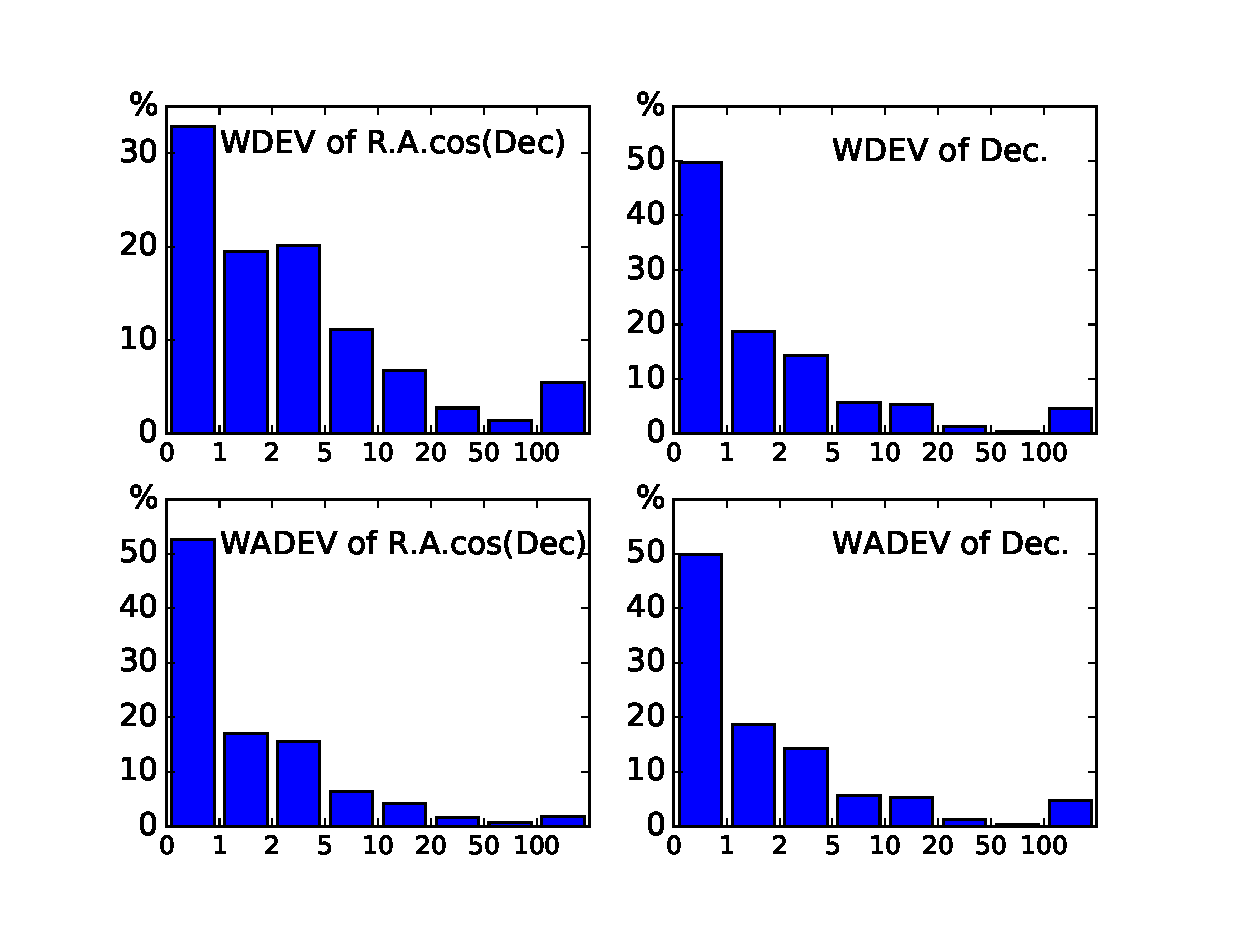
\includegraphics[width=\hsize]{figures/DEV_plot.eps}
      \caption{
      The statistical histograms of the weighted standard deviation (WDEV) and the weighted Allan deviation (WADEV) for $\alpha\cos\delta$ ($left$) and $\delta$ ($right$) coordinates. The units are mas.
              }
         \label{Fig:Dev}
\end{figure}

\begin{figure}
   \centering
   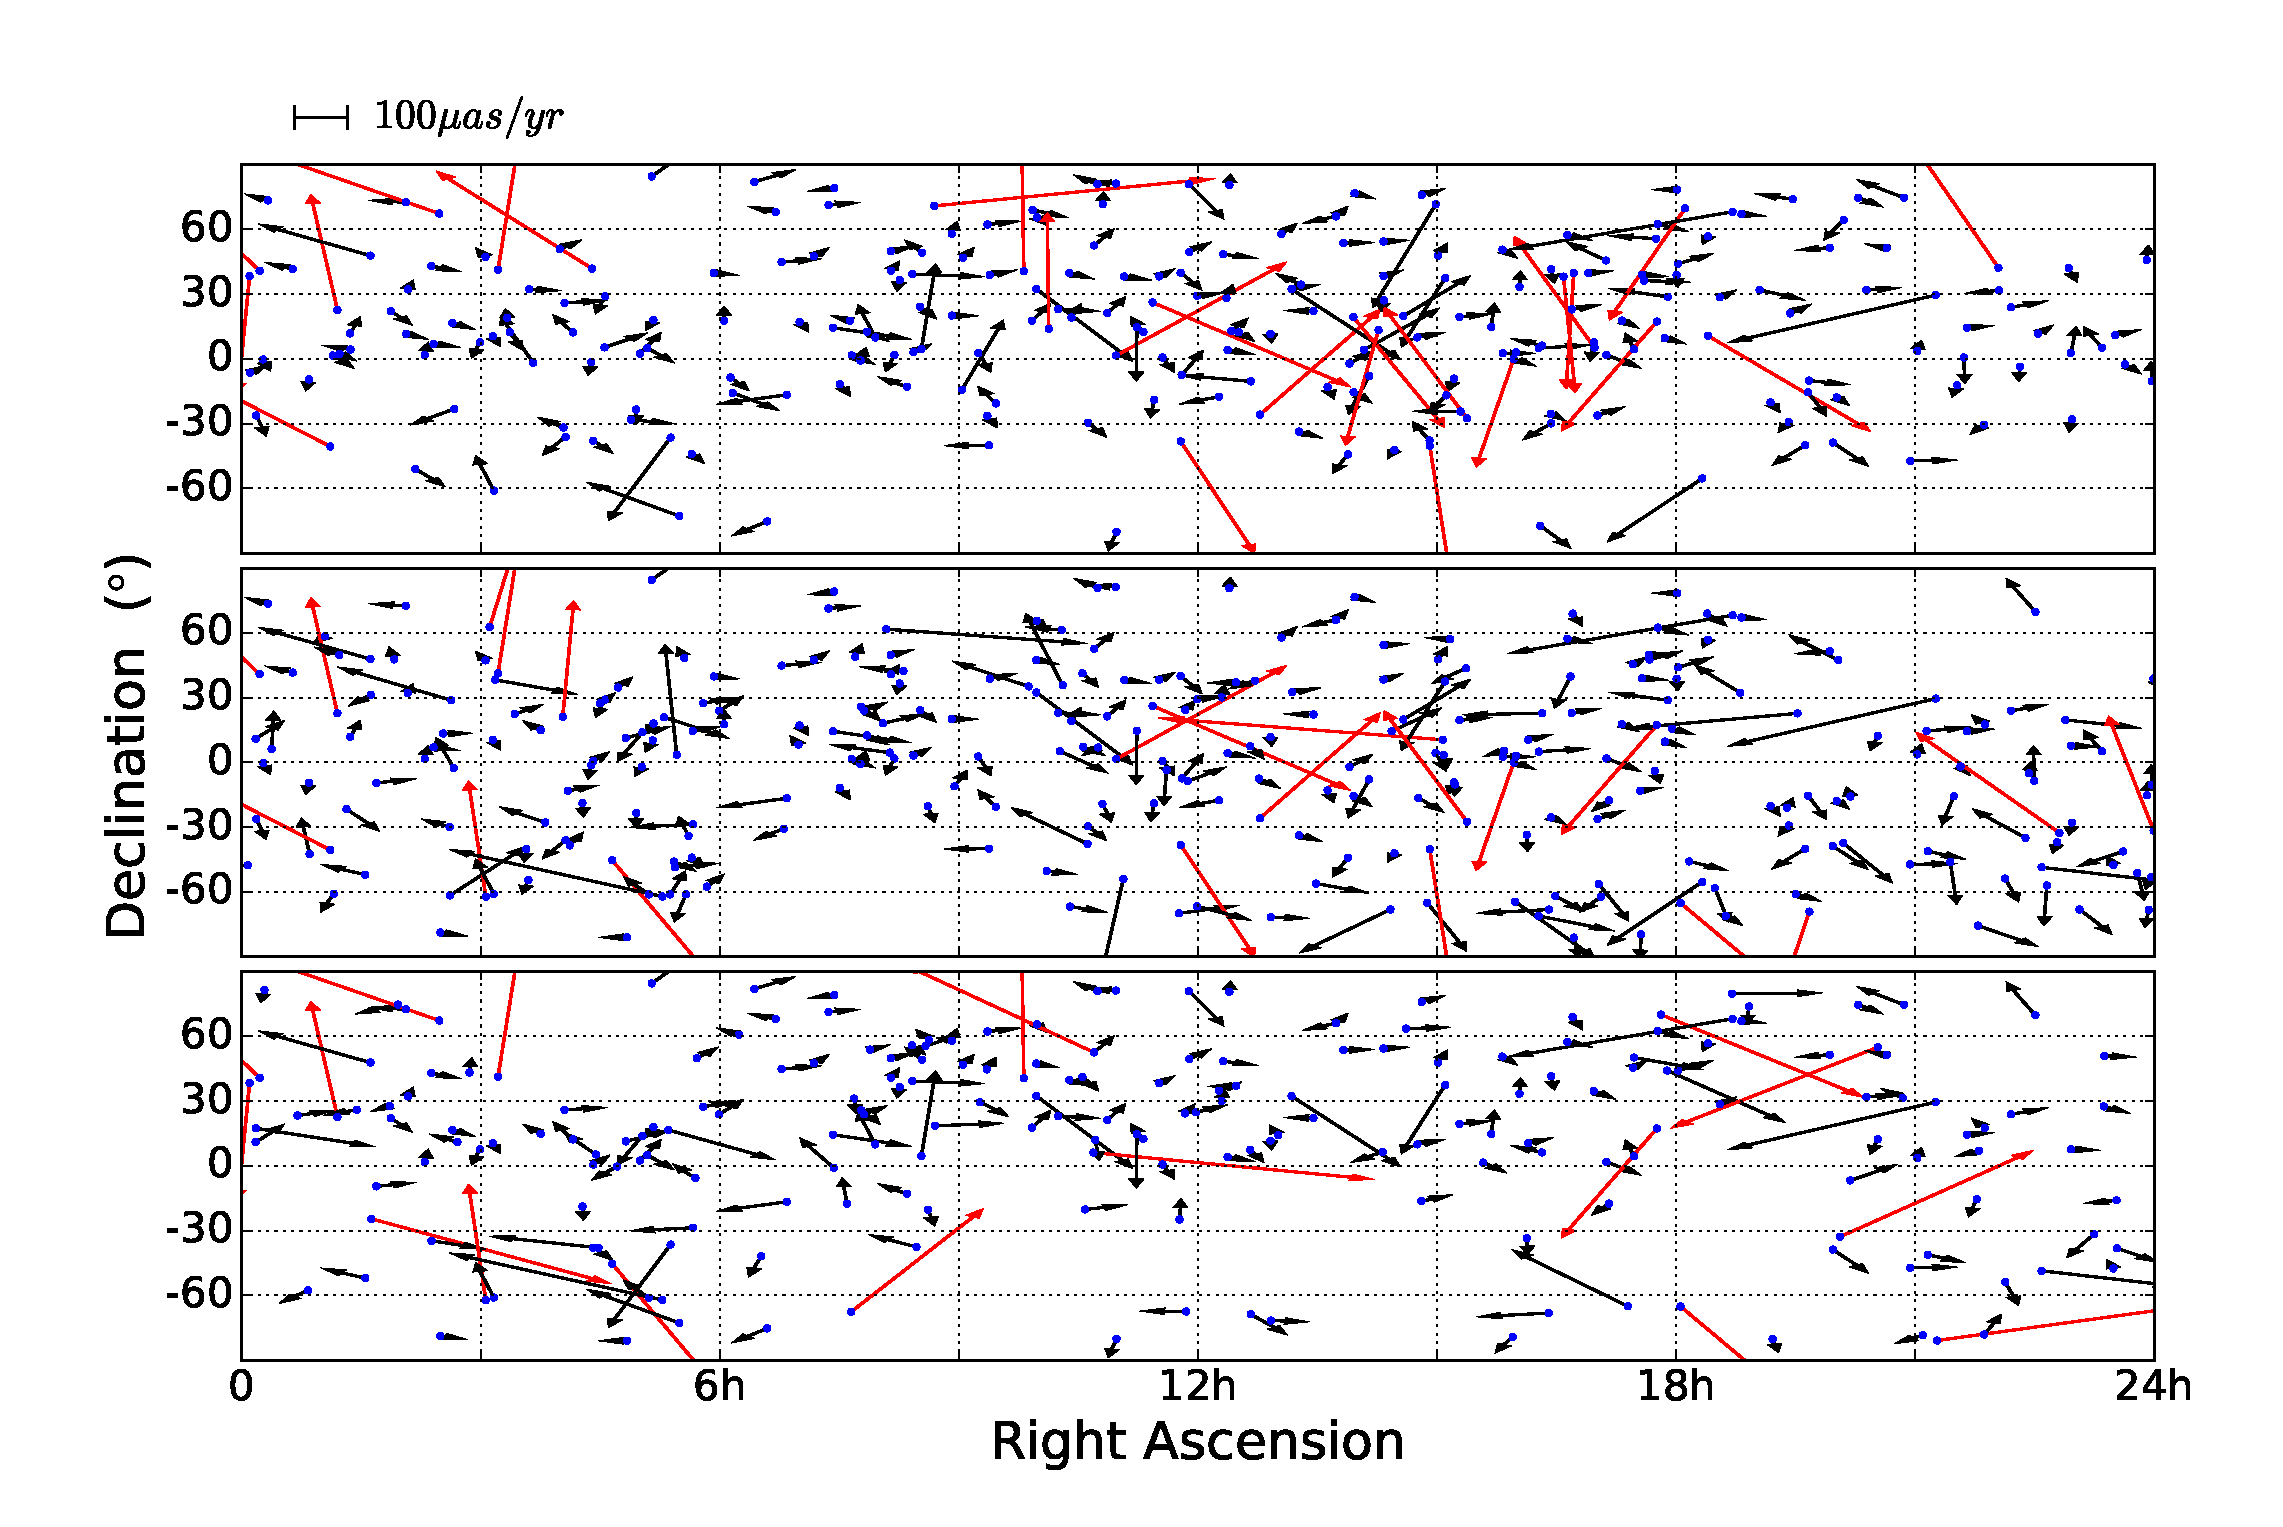
\includegraphics[scale=0.3]{figures/Linear_drift_3.eps}
      \caption{
      Linear drift of sources in three subsets: 212 ICRF($bottom$), 295 ICRF($middle$) and 247 MFV($top$). The linear drift larger than 500 $\mu as\cdot yr^{-1}$ is adjusted to 500 $\mu as\cdot yr^{-1}$ and plotted in red arrow.
              }
         \label{Fig:Ld3}
   \end{figure}

%
\subsection{Considerations on the axial stability}
The stability or inertia of a reference frame axes is usually assessed by the amplitude of global rotation vector $\vec{r}=(r_1,r_2,r_3)^{\rm T}$, where $r_1$, $r_2$, and $r_3$ are derived by least squares fit of source linear drifts to the following equations:
\begin{eqnarray}\label{eq:rotation}
      \mu_{\alpha}\cos\delta & = & +r_1\cos\alpha\sin\delta +r_2\sin\alpha\sin\delta -r_3\cos\delta \nonumber \\
      \mu_{\delta} & = & -r_1\sin\alpha + r_2\cos\alpha.
\end{eqnarray}
Note that some additional parameters such as slopes in right ascension and declination ${\rm d}z$ are occasionally estimated simultaneously \citep[for example]{Lambert2013} for specific purposes, however we only take global rotation into account since it is sufficient to estimate the stability of the reference frame.

Fig. \ref{Fig:rot_num} shows the evolution of $r_1, r_2, r_3$ and $r = |\vec r|$ with the number of picked sources from the ''Overall rank list" and the ''Partition rank list", respectively. It can be obviously seen from the trend that as the number increases, more sources with large linear drift $\mu$ are included, which cause more significant axial rotations.  Eclipses and peaks in the curve are also visible. For the two original rank list, $r$ is approximately equal when the number of sources is below 500. The level of $r$ is smaller than that for 295ICRF by a factor of two.

In fact, the first order vector spherical harmonics should include glide pattern besides global rotation \citep{Mignard2012}. The glide $\vec{d}=(d_1,d_2,g_3)$ are estimated together with $\vec r$ using the following equations:
\begin{eqnarray}
      \mu_{\alpha}\cos\delta & =& -d_1\sin\alpha + d_2\cos\alpha    \nonumber                   \\
                         &   & +r_1\cos\alpha\sin\delta +r_2\sin\alpha\sin\delta -r_3\cos\delta \nonumber  \\
      \mu_{\delta}           & =& -d_1\cos\alpha\sin\delta -d_2\sin\alpha\sin\delta +d_3\cos\delta  \nonumber  \\					                     &   & -r_1\sin\alpha + r_2\cos\alpha.
   \end{eqnarray}

Figure \ref{Fig:Rot_Gli} displays the values for the components and amplitudes of $\vec r$ and $\vec d$ as the selected sources increase. The figures show that the rotation part is close to the one in previous case (c.f. Fig. \ref{Fig:rot_num}), while the magnitude of glide keeps nearly unchanged. For this reason we only consider rotation part. Higher order of harmonics are not considered due to the smallness of the coefficients and insufficient source numbers.

\begin{figure}
   \centering
   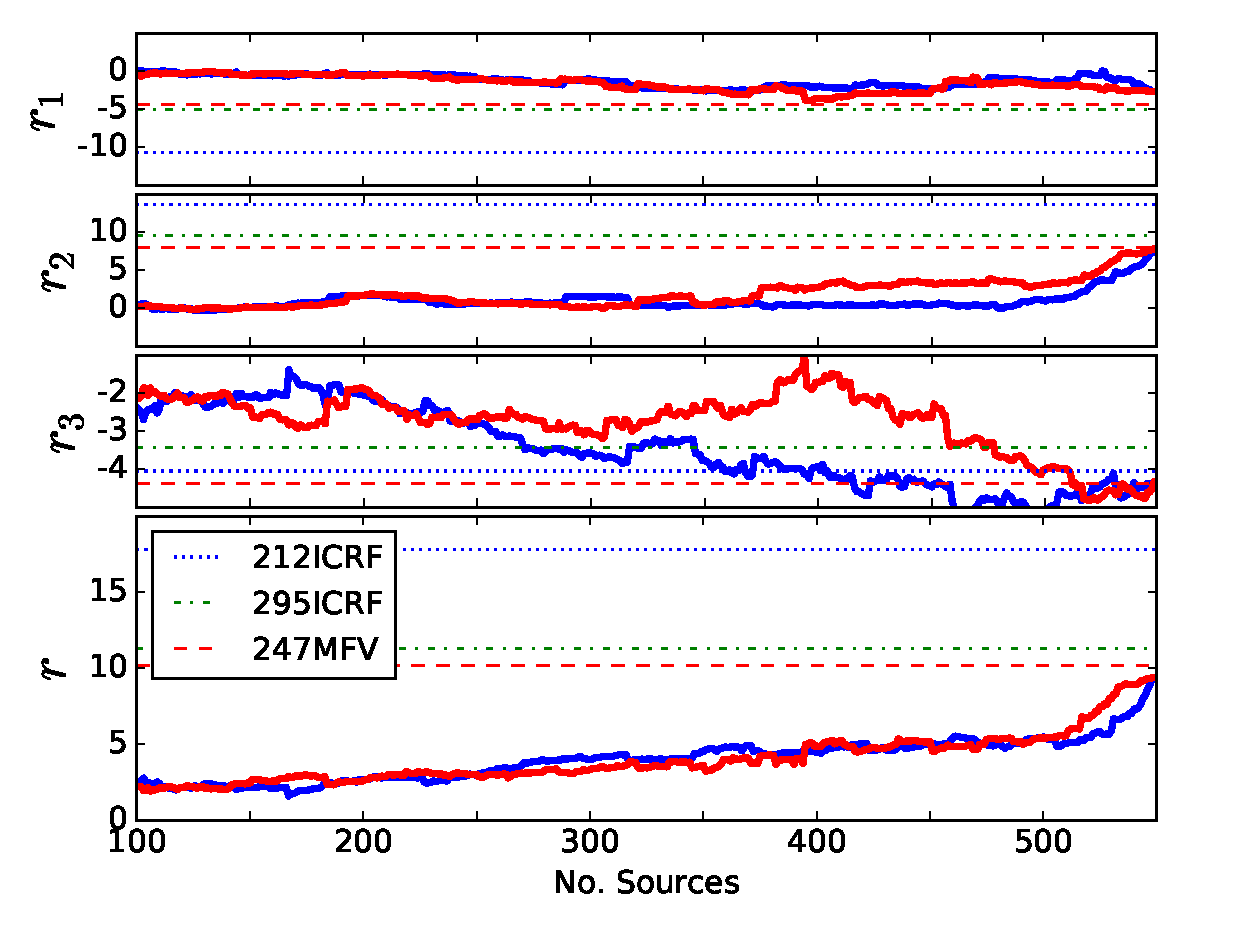
\includegraphics[scale=0.5]{figures/Rot_num.eps}
      \caption{
      The fitting results of rotation vector of the Overall Rank ($blue$) and Partition Rank ($red$) list. The three horizontal lines are the results of the three special subsets, as given in the legend.
              }
         \label{Fig:rot_num}
\end{figure}

	\begin{figure}
   \centering
   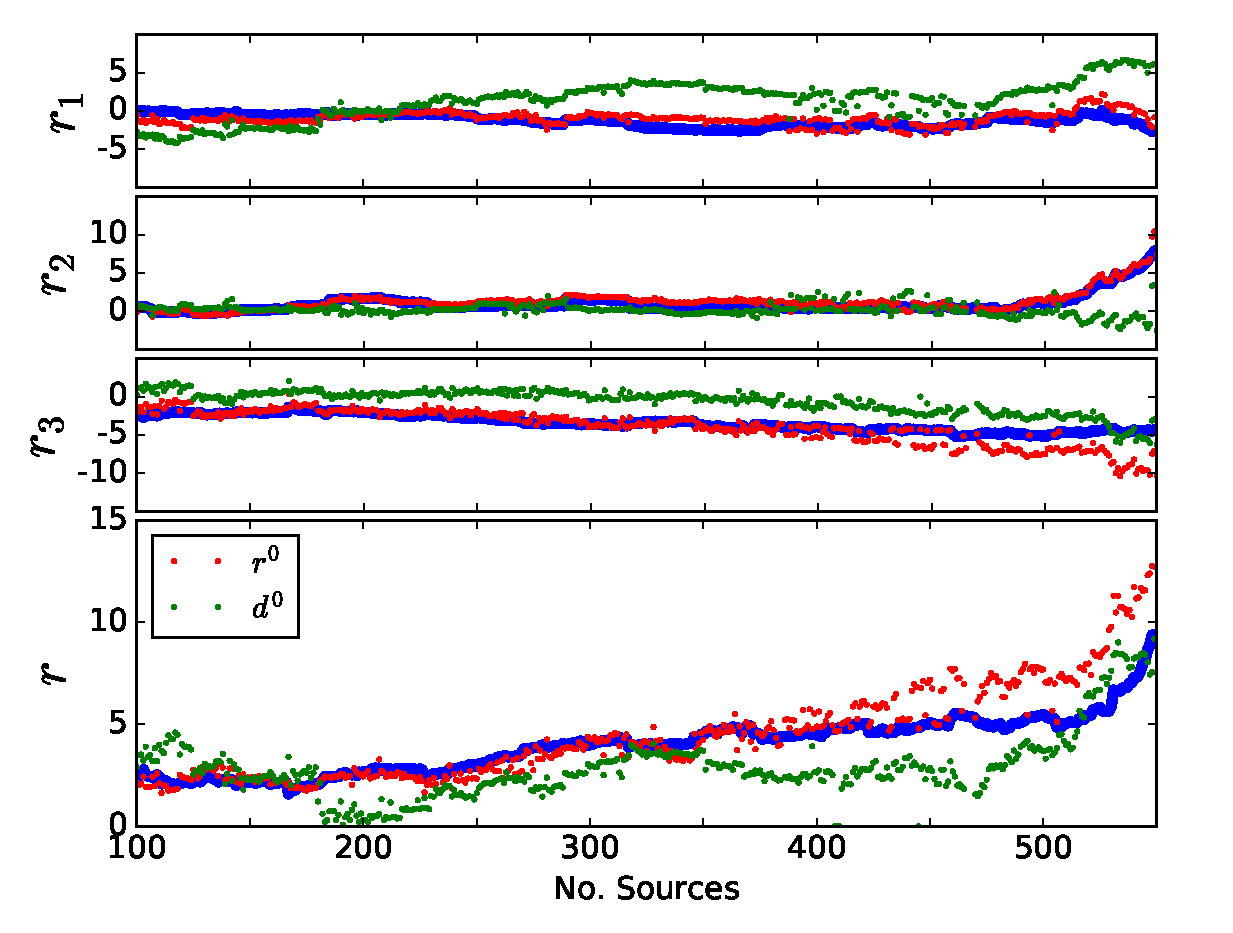
\includegraphics[width=\hsize]{figures/Rot_Gli.eps}
      \caption{
      The fitting results of considering rotation and glide vector both. The blue line is the result shown in Fig . The red and green point are corresponding part of rotation and glide respectively. The rank list is Overall Rank list.}
      \label{Fig:Rot_Gli}
   \end{figure}

\subsection{Considerations On the sky distribution}
The level of uniform for the sources distribution on the celestial sphere is another aspect that need to be assessed. The mean declination of subset is one of index for such purpose. \citep{Liu2012} provided an approximate approach to assess uniformity of source distribution. In that method, a dipolar vector field are generated based on the coordinates of sources with an assumed amplitude, then global rotation (denoted $\vec g$) fitted with Eq. \ref{eq:rotation} is used as the parameter for describing the homogeneity of the distribution. It is shown that an ideal uniform ensemble of sources will give a zero rotation. The simulation is applied but the direction of the dipolar vector field is set to be the North celestial pole instead of the Galactic center.

Fig. \ref{Fig:sim} shows the result of simulation.
%When the number of sources is smaller than 400,
	\begin{figure}
   \centering
   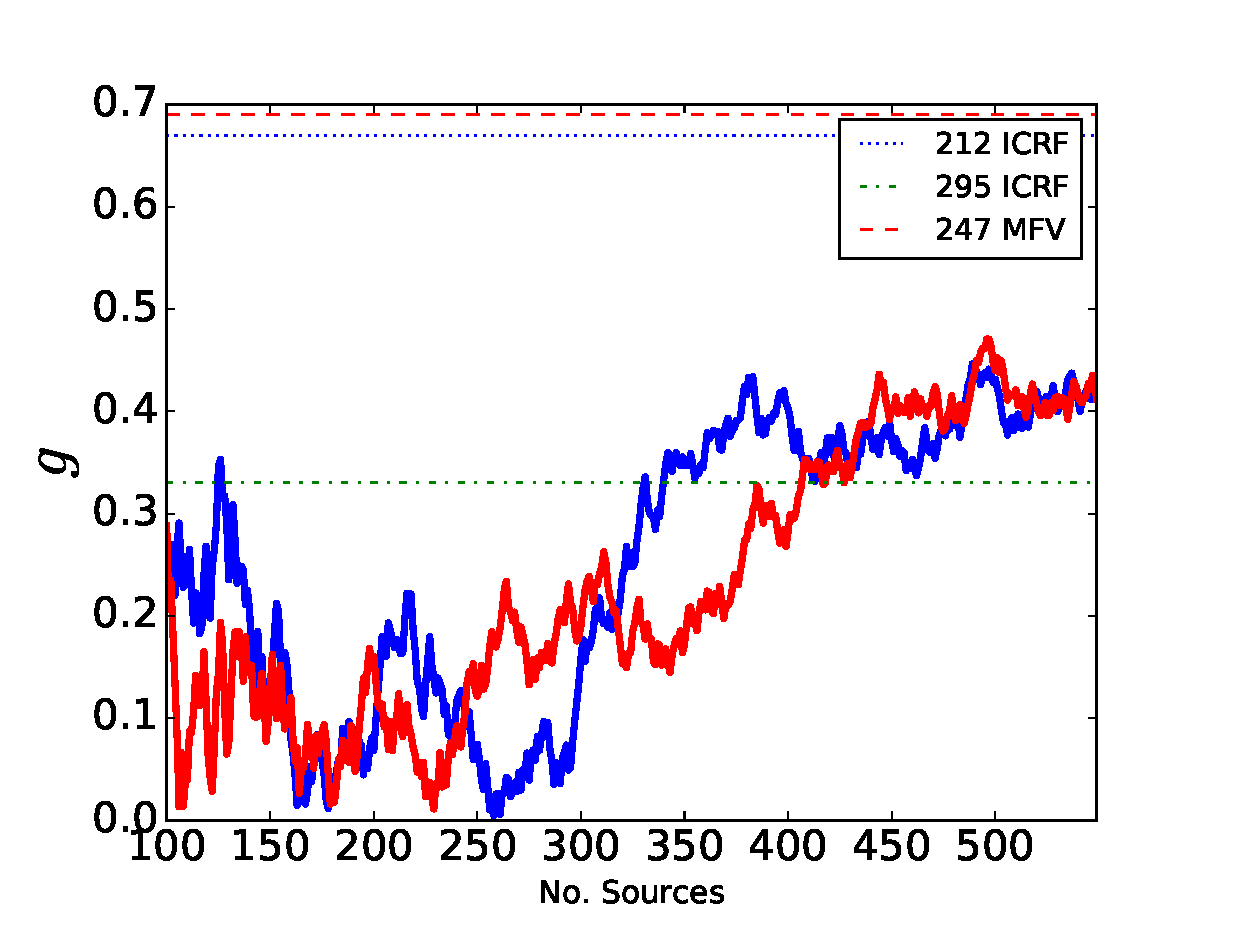
\includegraphics[width=\hsize]{figures/Simulation.eps}
      \caption{
      The results of simulation. The blue and red line are corresponding result of rank1 and rank2 respectively.
              }
         \label{Fig:sim}
   \end{figure}

\subsection{Consideration on above two respects}
When considerations on axial stability and sky distribution are taken simultaneously, a quality index of selected source list is defined as
\begin{equation}
Q = \frac{3r_N+g_N}{4},
\end{equation}
where $r_N$ and $g_N$ are the results of Fig. \ref{Fig:rot_num} and \ref{Fig:sim} normalized to unit. This weight ratio 3 shows a priori consideration on axial ability compared to distribution. The result of Q for different selections are given in Fig. \ref{Fig:com_num} and four ensembles of sources with sources among 300-400 are finally selected (pointed out by red triangles) and were called "Sou322", "Sou351", "Sou371", and "Sou394". The linear drift of sources in these four sets are shown in Fig. \ref{Fig:Ld4}, most sources showing insigficant linear drift and a good sky coverage. And the corresponding statical information is given in Table.  \ref{Tab:Mean_Dec}, and Table.\ref{Tab:Axi}.

	\begin{table}
	\caption{Mean declinations for our selected source lists.}
	\label{Tab:Mean_Dec}
	\centering
	\begin{tabular}{ccc}
	\hline\hline
List & Mean declination  &No. of 295ICRF sources         \\
\hline
Sou322& -0.13$^{\circ}$ &140                 \\
Sou351& -0.37$^{\circ}$ &154                 \\
Sou371& -0.48$^{\circ}$ &163                 \\
Sou394& -0.51$^{\circ}$ &173                 \\
\hline
	\end{tabular}
	\tablefoot{The mean declination for 212 ICRF, 295 ICRF2 and 247 MFV are 4.80$^{\circ}$, 0.70$^{\circ}$, and 16.89$^{\circ}$ respectively.}
	\end{table}
	
	\begin{table}
	\centering
	\caption{Fitted global rotations for our selected source lists. The unit is  $\mu \rm{as \, yr}^{-1} $}
	\label{Tab:Axi}	
	\begin{tabular}{ccccc}
\hline\hline
List    &$r_1$          &$r_2$          &$r_3$          &$r$    \\
\hline
Sou322 &-1.7$\pm$0.3 &1.1$\pm$0.3 &-2.8$\pm$0.3 &3.4$\pm$0.5 \\
Sou351 &-2.3$\pm$0.3 &0.5$\pm$0.3 &-2.2$\pm$0.3 &3.2$\pm$0.4 \\
Sou371 &-2.4$\pm$0.2 &1.6$\pm$0.2 &1.6$\pm$0.2 &3.7$\pm$0.4 \\
Sou394 &-2.7$\pm$0.2 &2.4$\pm$0.2 &-1.0$\pm$0.2 &3.8$\pm$0.4 \\
\hline
	\end{tabular}
	\end{table}	
	


	\begin{figure}
   \centering
   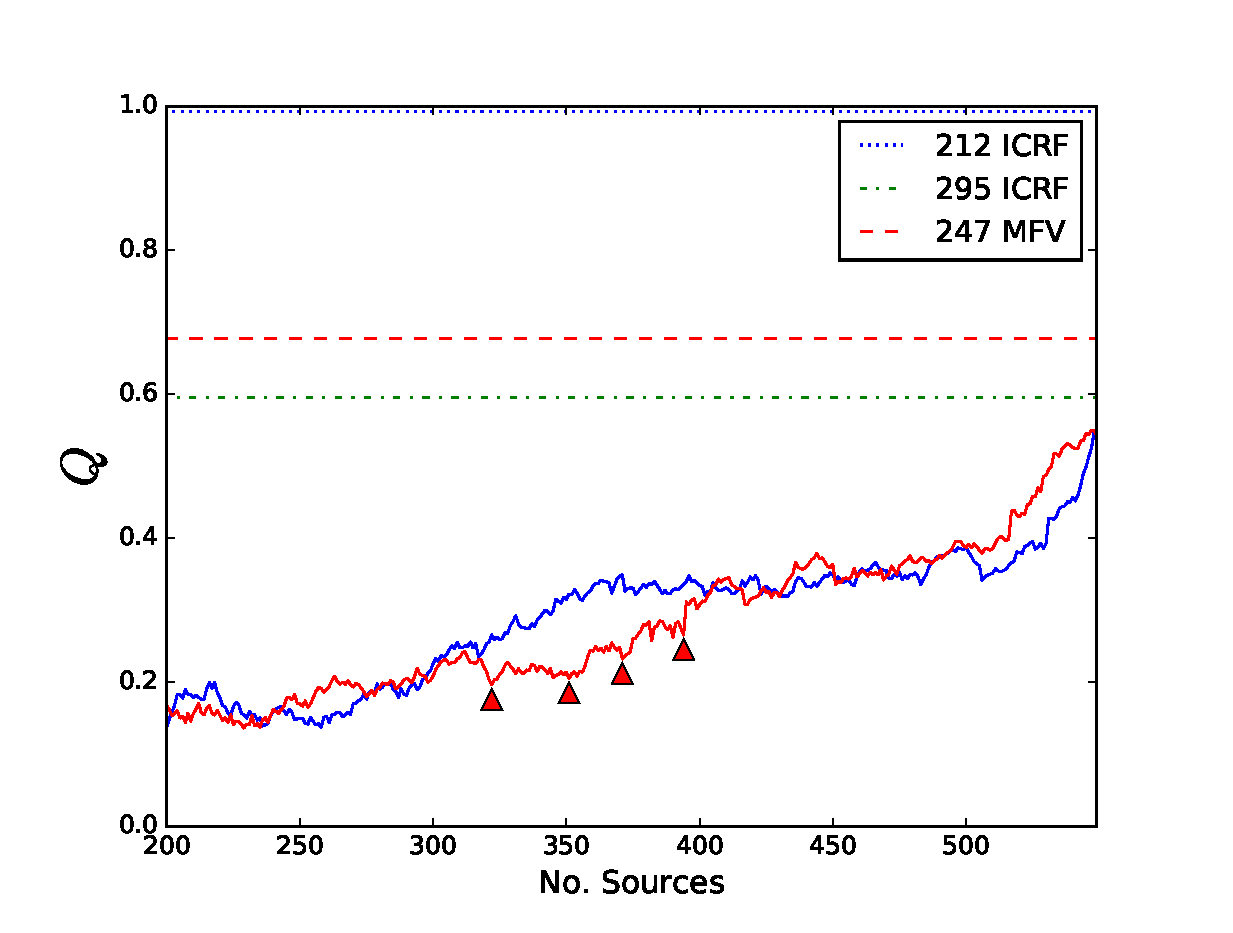
\includegraphics[width=\hsize]{figures/Quality.eps}
      \caption{
      The Quality index for different source list according the number. The final selections are labeled by red triangles.
              }\label{Fig:com_num}
   \end{figure}

   \begin{figure}
   \centering
	 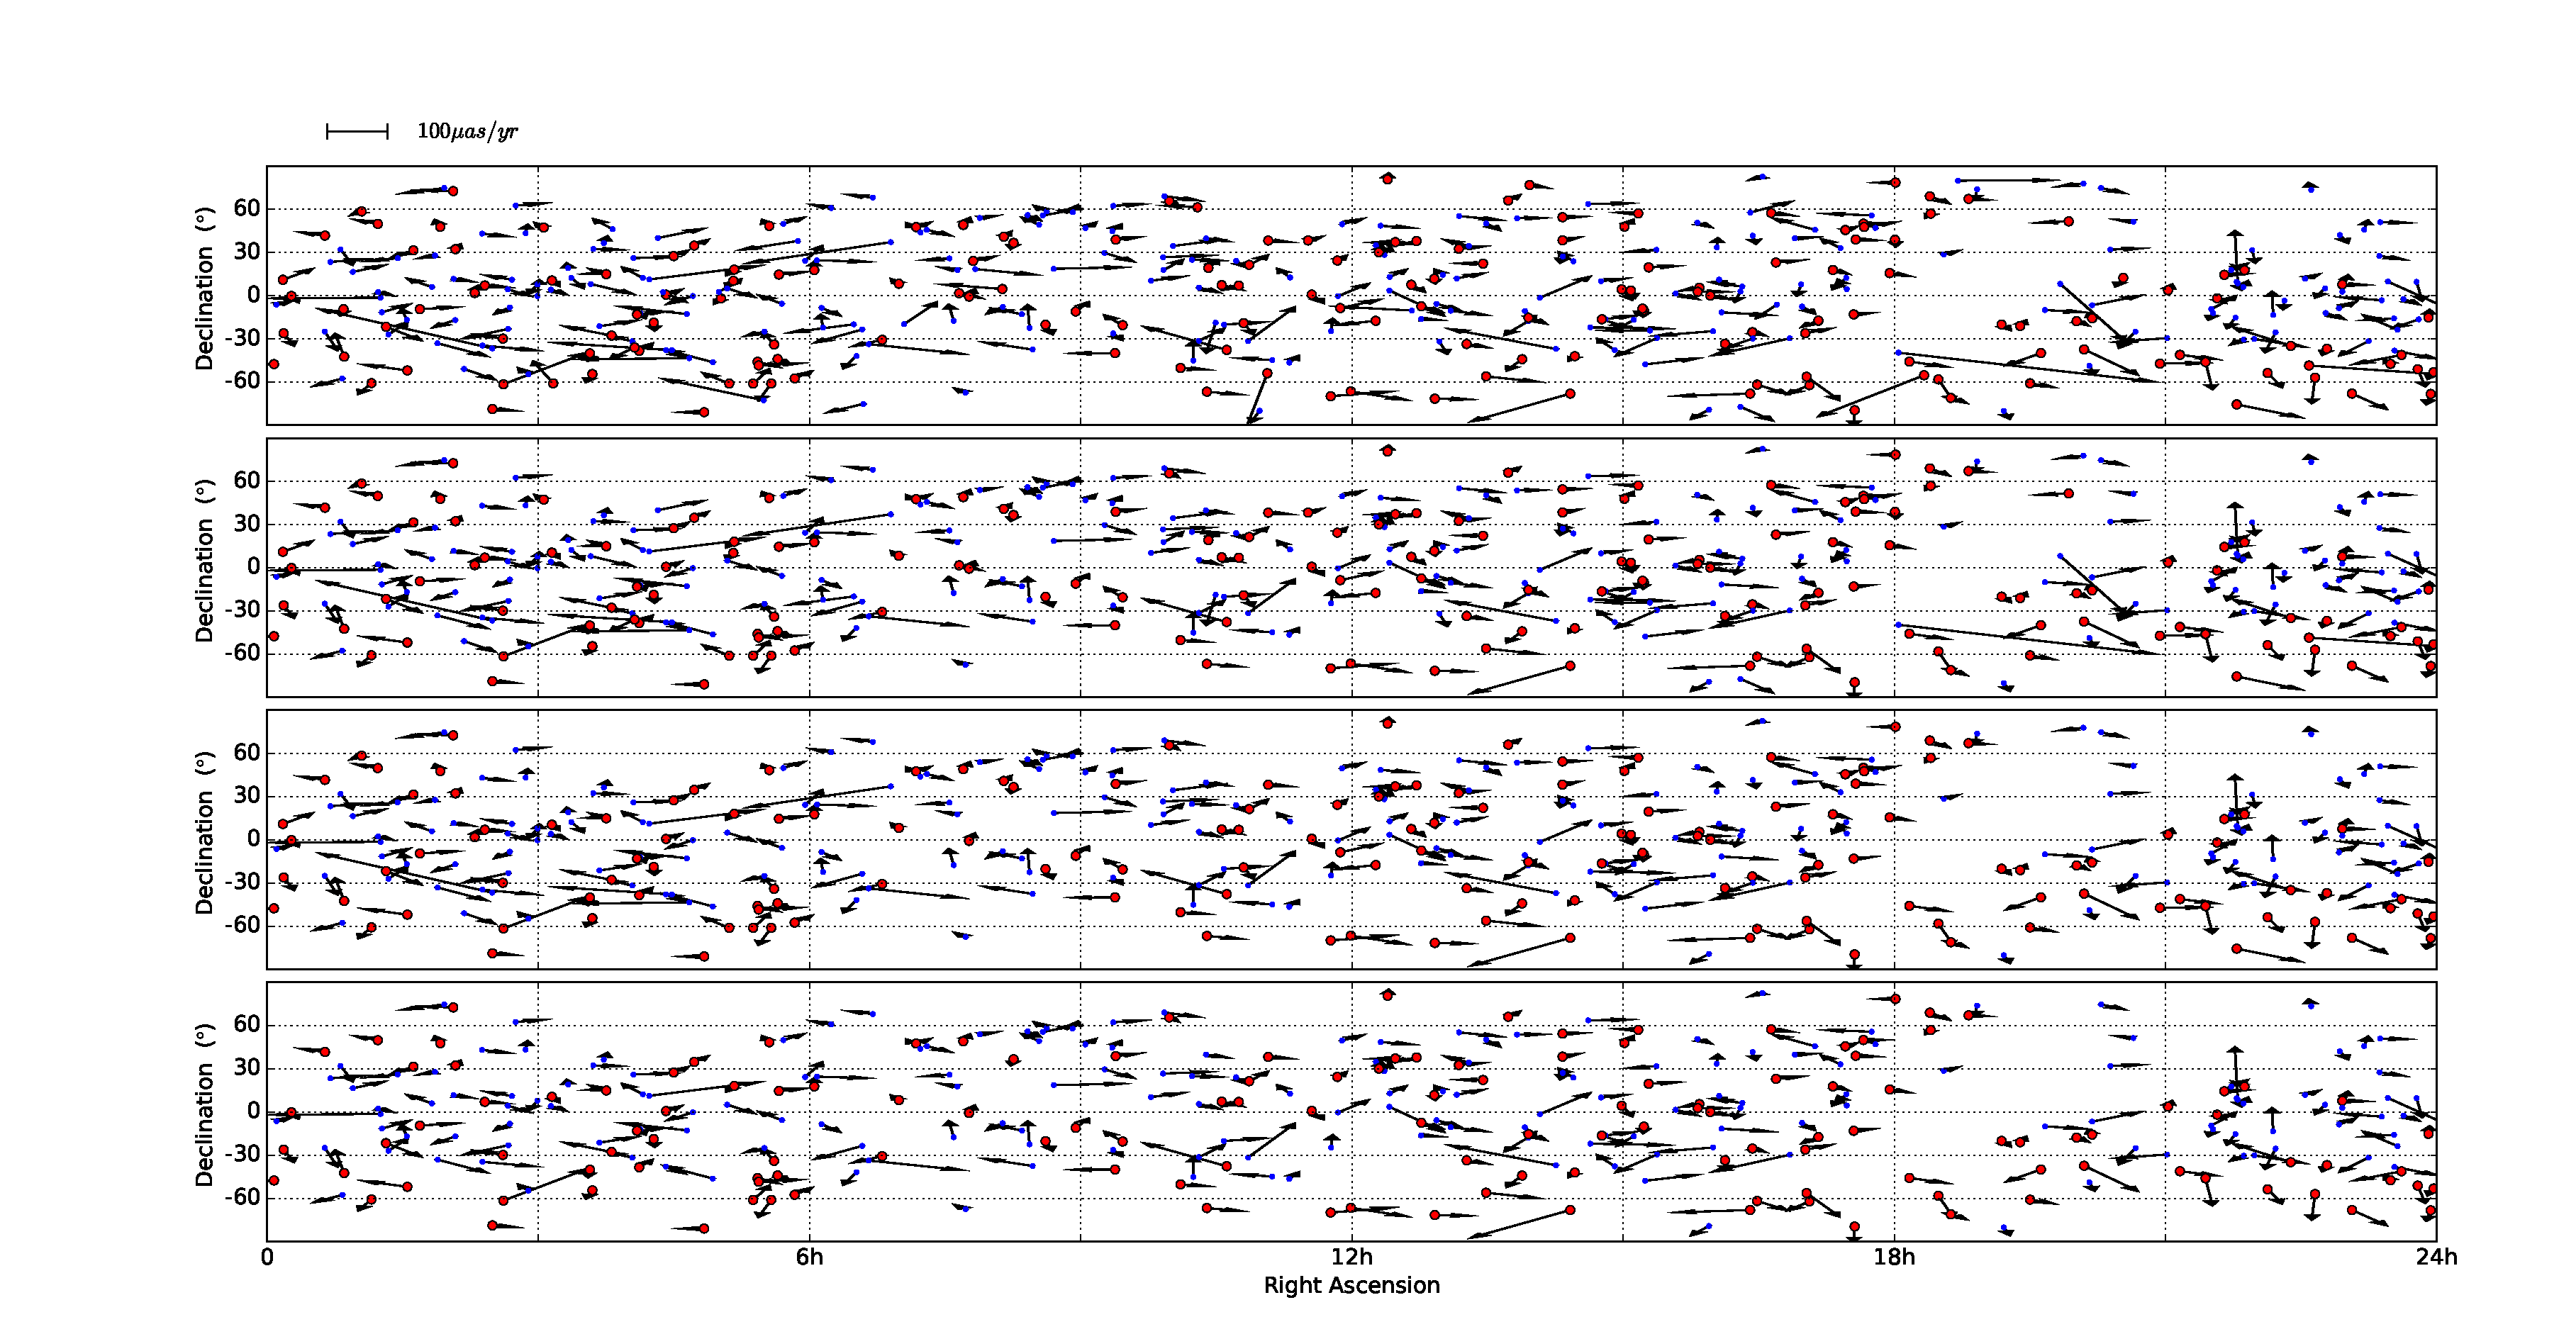
\includegraphics[scale=0.3]{figures/Linear_drift_4.eps}
      \caption{
      Linear drift of four sets of sources to be considered as defining sources. The red points means that the sources is included in ICRF2 defining sources.
              }
         \label{Fig:Ld4}
   \end{figure}
%-----------------------------------------------------------------
\section{Conclusions}\label{sect:conclusion}
With the time series of coordinates over 30 years for sources, some of ICRF2 defining appear to be unstable and not suitable to defining a celestial frame. 4 sets of sources with improved in both axial stability and uniform sky distribution are recommended.
%-----------------------------------------------------------------

%\begin{acknowledgements}
%
%\end{acknowledgements}

\bibliographystyle{aa}
\bibliography{bibtex/SourcesSelection}
\end{document}
